\subsection{Informatik}

\author{Alexander Suter}

\begin{frame}
	\frametitle{Übersicht\hfill{}\footnotesize \group}

		\begin{figure}
			\centering
			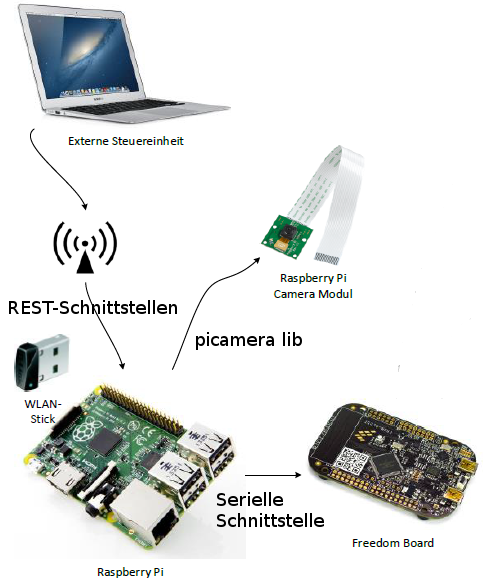
\includegraphics[width=0.5\textwidth]{../../fig/blockdiagramm-informatik.png}
		\end{figure}
		
		% Nun zum Informatik Teil. Auf dieser Folie sehen
		% Sie eine Übersicht. Ich werde nun diese Grafik erklären
		% und dannach konkret auf die einzelnen Komponenten eingehen.
		
		% Die Informatik deckt zwei Anforderungen ab. Das Senden
		% und Empfangen des Start- und Stoppsignals - drathlos.
		% Und die Ortung des Korbes.
		
		% Wie auf der Grafik zu erkennen. Zentral ist das Pi, welches % auch die gesamte Maschinerie steuert. Das Pi stellt einen
		% Access-Point zur Verfügung. Die externe Steuerungseinheit, 
		% in unserem Fall das Notebook, verbindet sich mit dem Pi. 
		% Und so steht uns hier der TCP/IP Stack zur Verfügung.
		
		% Das Pi hat die für die zweite Anforderung eine Kamera.
		% Diese Kamera ist über CSI (Camera Serial Interface) macht % ein Foto des Korbes und mithilfe eines
		% selbst programmierten Algorithmus auf dem Pi wird der Ort
		% bzw. der Winkel berechnet.
		
		% Über eine serielle Schnittstelle ist das Freedom Board
		% verbunden, welches für die Steuerung und Regelung der 
		% Motoren zuständig ist.
		
		% Auf dem Pi wird mit Python gearbeitet. Die Entscheidung
		% ist schon früh gefallen, da der Zugriff auf die serielle
		% Schnittstelle mittels Python ein Leichtes ist.
		% Wir haben dann geprüft ob wir mittels Python eine REST
		% Schnittstlele implementieren können und die Kamera ansprechen.
		% Für beides haben wir bewährte Librarys gefunden und auch
		% die Bildverarbeitung ist mittels Python möglich.

\end{frame}

\subsubsection{Bordcomputer}
\begin{frame}
	\frametitle{Bordcomputer\hfill{}\footnotesize \group}
	\framesubtitle{Raspberry Pi}
	
	\begin{columns}
		\begin{column}{0.5\textwidth}
			\begin{figure}
				\centering
				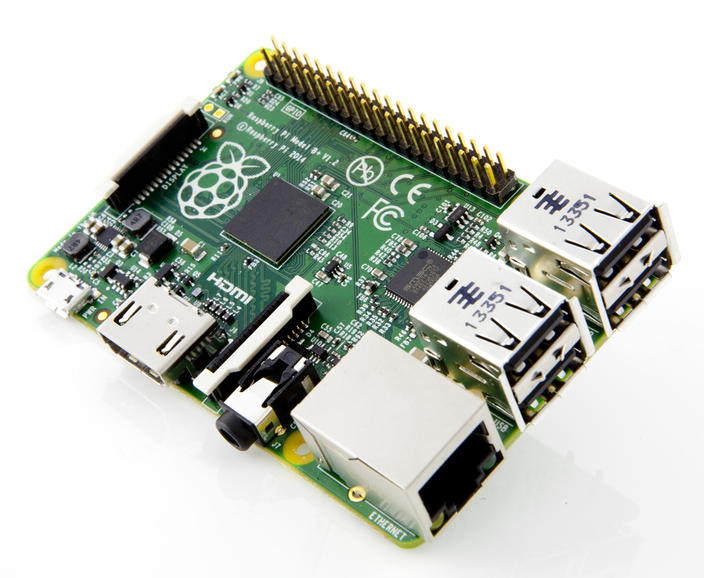
\includegraphics[width=0.8\textwidth]{../../fig/raspberry-pi-b-plus.jpg}
				\caption{Raspberry Pi (B+)}
			\end{figure}
		\end{column}
		\begin{column}{0.5\textwidth}
			\begin{block}{Spezifikation}
				\begin{itemize}
					\item CPU: 700Mhz Broadcom BCM2835
					\item RAM: 512 MB
					\item 4 USB Ports
					\item Micro SD Slot (8GB)
					\item CSI Schnittstelle
				\end{itemize}
			\end{block}
		\end{column}
	\end{columns}
	
    % Ervin hat bereits erklärt warum wir uns für das Pi entschieden
    % haben.
    
    % Die relevante Spezifikation für das Pi ist folgende:
    % 700Mhz, 512Mb RAM - entscheidend für die Bildverarbeitung
    % 4 USB Ports -> WLAN-USB Stick eventuell offen für bessere CAM
    % Micro SD Slot 8GB (Betriebssystem 64MB RAM, 800MB Speicherplatz, % Pyhton, unser Source code)
    % CSI Schnittstelle für die Kamera.
    
    % Falls die Rechenpower doch nicht ausreicht, können wir schnell
    % eine REST-SST erstellen und Berechnungungen um so Berechnungen
    % auf das Mainframe auszulagern.
	
\end{frame}

\subsubsection{Bildverarbeitung}
\begin{frame}
	\frametitle{Bildverarbeitung\hfill{}\footnotesize \group}
	\framesubtitle{Kamera}
	
	\begin{columns}
		\begin{column}{0.5\textwidth}
			\begin{figure}
				\centering
				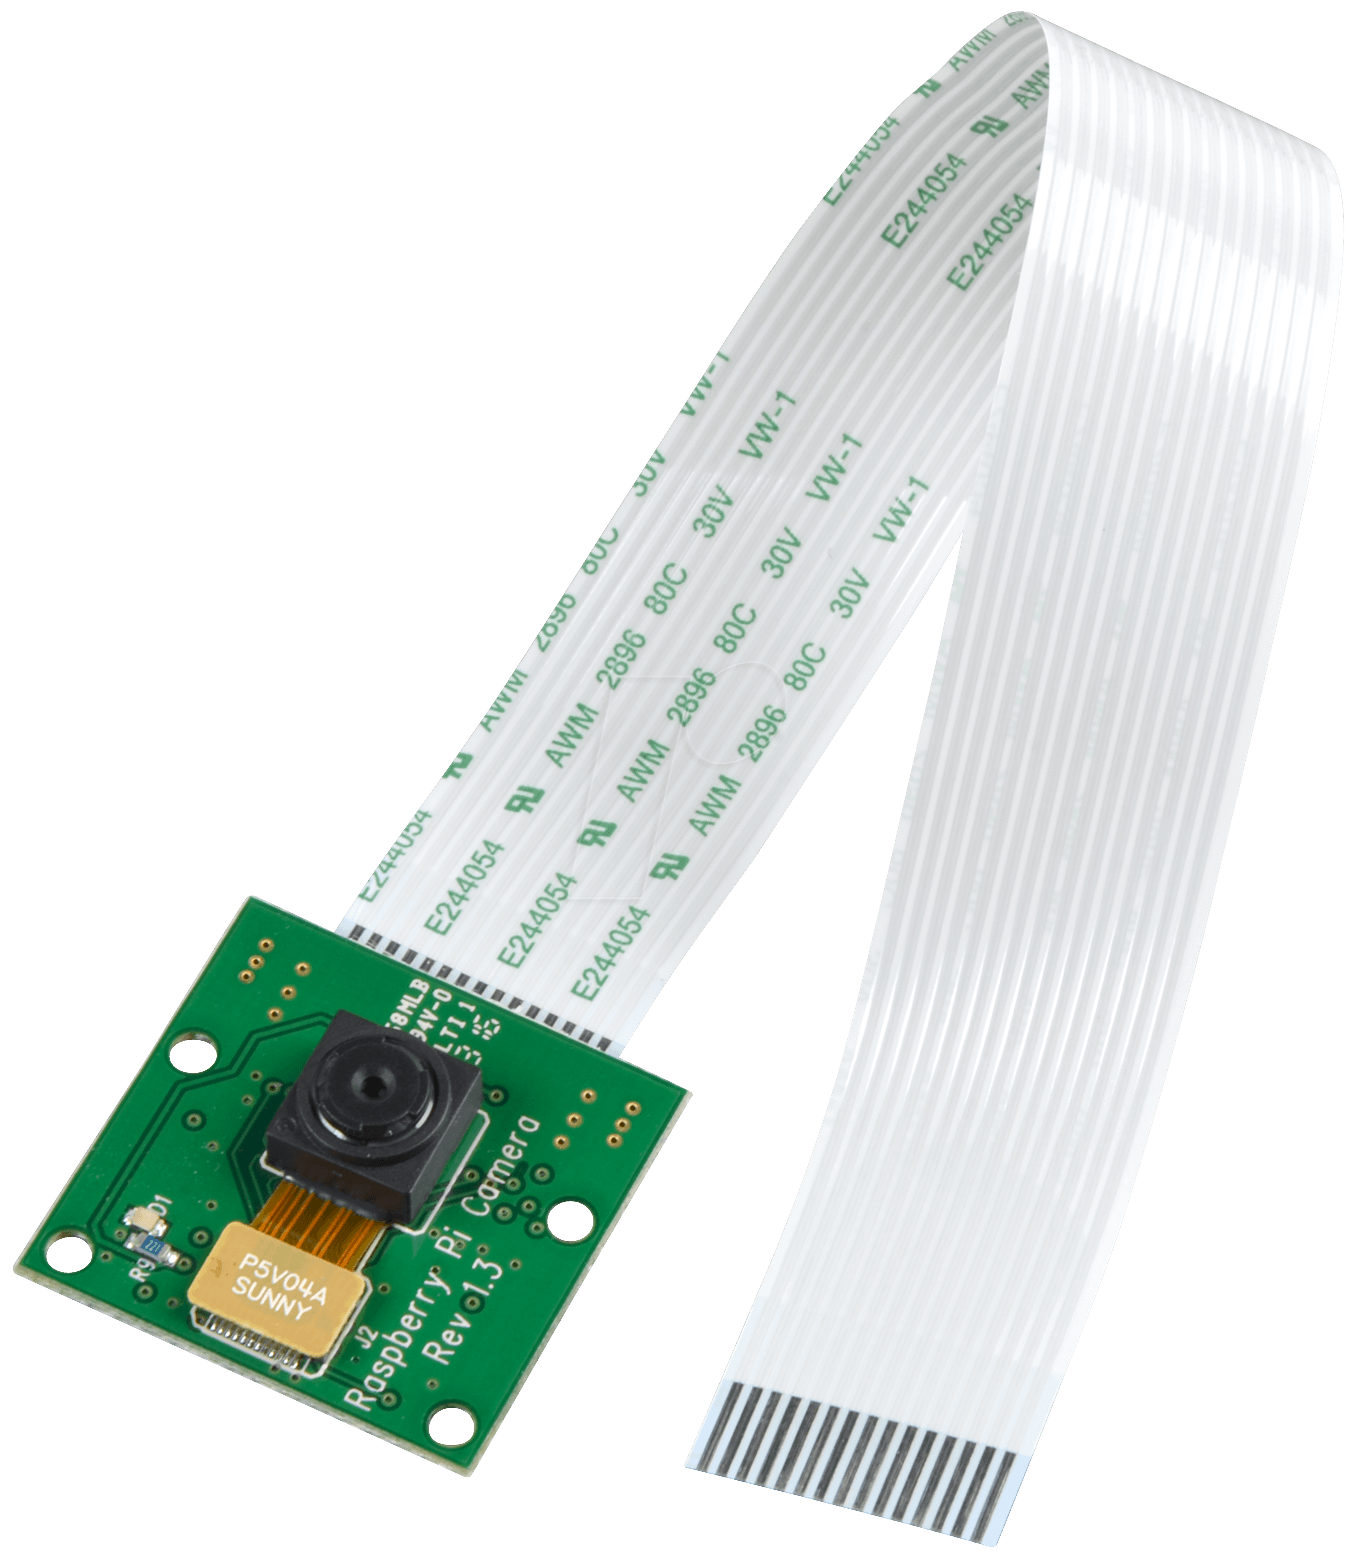
\includegraphics[width=1\textwidth]{../../fig/raspberry_pi_cam.png}
				\caption{Raspberry Pi Camera}
			\end{figure}
		\end{column}
		
		\begin{column}{0.5\textwidth}
			\begin{block}{Spezifikation}
				\begin{itemize}
					\item Horizontales Sichtfeld: 53 Grad
					\item Vertikales Sichtfeld: 40 Grad
					\item Auf einer Distanz von 2 Meter entspricht das eine Fläche = 2m X 1.3m
					\item Ansteuerung über CLI oder Python Picamera.
				\end{itemize}
			\end{block}
		\end{column}
		
	\end{columns}
	
	% Das Produkt aus dem Hause Raspberryi. Verbunden über eine
	% standardisierte Schnittstelle CSI. Daher werden in diesem
	% Bereich mit grosser Wahrscheinlichkeit überhaupt keine Probleme
	% auftreten. 
	% Wir haben geprüft ob das Sichtfeld der Kamera auch wirklich
	% die gesamte Wand abdeckt. Unsere Berechnungen haben ergeben
	% dass auf einer Distanz von 2 Metern - eine Fläche von 2m
	% in der Breite und 1.3 Metern in der Höhe abgedeckt werden kann.
	
\end{frame}

\begin{frame}
	\frametitle{Bildverarbeitung\hfill{}\footnotesize \group}
	\framesubtitle{Algorithmen zur Informationsauswertung}
	
	\begin{figure}
		\centering
		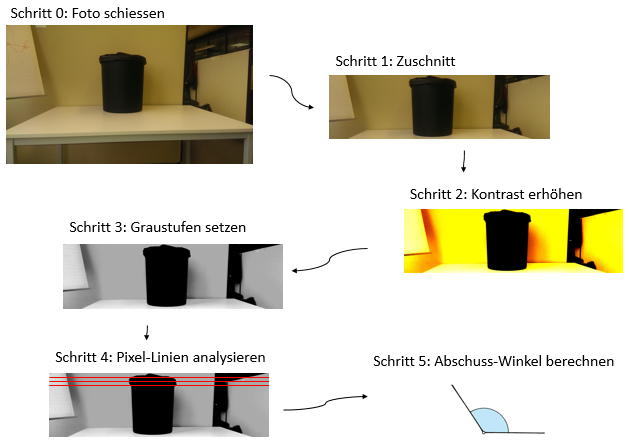
\includegraphics[width=0.8\textwidth]{../../fig/ablauf-ortung-des-korbes-algorithmus.png}
	\end{figure}
	
	% Algorithmus erklären und was die einzelnen
	% Schritte auch technisch machen.
	
	% Zudem noch die Helligkeit und der Weissablgeich
	% ansprechen.

	% Helligkeit erhöhen - es werden mehr Kanten ersichtlich.
	% Weissabgleich dient dazu die Kamera auf die Farbtemperatur
		% des Lichtes am Aufnahmeort zu sensibilisieren. Bspw.
		% um rot -und blau stiche zu vermeiden.
	
\end{frame}

\begin{frame}
	\frametitle{Bildverarbeitung\hfill{}\footnotesize \group}
	\framesubtitle{Parametrierung des Algorithmus}
	
	\begin{figure}
		\centering
		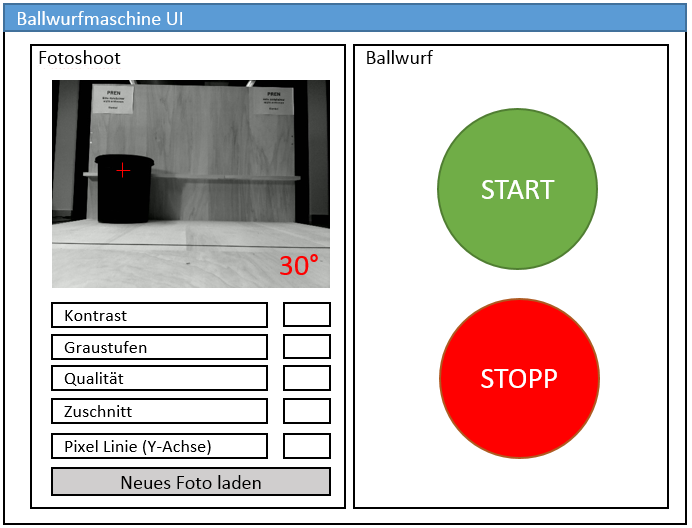
\includegraphics[width=0.6\textwidth]{../../fig/fotoshoot-configurator.png}
		\caption{Ballwurfmaschine UI}
	\end{figure}
	
	% UI um den Algorithmus in der Vorbereitung anzupassen.
	% Start-Stopp Signal.
	% Parameter Konfigurierbar - auf externe Steuerungseinheit.
	% In Java.
	
\end{frame}
